% !TeX program = pdflatex
\documentclass{article}

\usepackage[utf8]{inputenc}
\usepackage[T1]{fontenc}
\usepackage{CJKutf8}
\usepackage[final]{neurips_2026}

\usepackage{hyperref}
\usepackage{booktabs}
\usepackage{amsfonts}
\usepackage{amsmath}
\usepackage{microtype}
\usepackage{graphicx}
\usepackage{subcaption}
\usepackage{xcolor}
\usepackage{pifont}
\usepackage{enumitem}
\usepackage{tabularx}
\usepackage{array}
\newcolumntype{Y}{>{\raggedright\arraybackslash}X}
\setlist{nosep,leftmargin=*}

\hypersetup{hidelinks}
\newcommand{\cmark}{\ding{51}}
\newcommand{\grade}[1]{\textbf{\textcolor{blue!70!black}{[#1]}}}

\graphicspath{{figures/}}

\renewenvironment{abstract}{%
  \centerline{\bfseries 摘要}\vspace{0.35em}\begin{quote}\small
}{%
  \end{quote}\vspace{0.6em}%
}
\renewenvironment{ack}{\section*{致谢}}{}

\title{CIFAR-10 上现代 ConvNet 的缩放规律与精度--效率权衡}

\author{%
  施博艺 \qquad 朱璞皓 \qquad 龚金烨 \\
  DD2424 深度学习与数据科学 · KTH · 小组 148 \\
}

\begin{document}
\begin{CJK}{UTF8}{gbsn}

\maketitle

\begin{abstract}
  在 CIFAR-10（$32{\times}32$）上，本文在匹配算力预算的前提下，比较 ConvNeXt 式 block 是否优于强 VGG 基线的精度--FLOPs 权衡。
  我们实现统一 PyTorch 管线（固定 45k/5k 训练/验证划分、AdamW、cosine+warmup、200 epoch、seed=42），完成计划实验 \textbf{17/17}：三族 block（VGG、深度可分离、ConvNeXt）在低（$\sim$150M）、中（$\sim$310M）、高（$\sim$460M）三档 FLOPs 下对齐 width，并扫描 kernel（$k{\in}\{3,5,7,11\}$）与 depth。
  \textbf{主要结果：}全局最优 \texttt{vgg\_baseline} $w{=}64$---309.5M FLOPs，test \textbf{92.78\%}；三档对齐后 VGG 均为最高；深度可分离在约 90\% VGG 算力下达 92.18\%（相当于 VGG 精度的 99.4\%）；ConvNeXt 在匹配预算下未超过 VGG/DW；kernel 增大对两族均为单调负收益（$k{=}11$ 较 $k{=}3$ 约降 3.7 pt）。
  我们给出 Pareto 前沿、单位 FLOP 边际收益与算力预算感知设计规则，并对照 Default Project 的 \grade{E}、\grade{D/C}、\grade{B/A} 任务。
\end{abstract}

\section{引言}

CIFAR-10 是 10 类、$32{\times}32$ 的标准分类基准。卷积网络从 VGG 式小卷积堆叠，演进到 MobileNet 式深度可分离卷积，再到 ConvNeXt 的大核 depthwise、LayerNorm 与倒瓶颈结构~\cite{liu2022convnext}。许多现代设计面向 ImageNet 分辨率；在低分辨率输入上，大感受野是否仍有净收益并不显然。

\textbf{默认配置比较的误导性。}$w{=}64$ 时，三族模板 FLOPs 分别为 309.5M（VGG）、40.4M（DW，仅为 VGG 的 13\%）、462.4M（CN，为 VGG 的 149\%）（表~\ref{tab:baseline}）。因此不能直接用默认 test 精度回答 RQ1，必须在\textbf{匹配算力}下比较，并系统扫描 width、kernel 与 depth。

\textbf{研究问题（小组 148 proposal）。}
\textbf{RQ1：}匹配 FLOPs 后，ConvNeXt 式 block 是否优于强 VGG 基线的 accuracy--FLOPs 权衡？
\textbf{RQ2：}depth、width、kernel、block 类型如何随预算缩放？哪一维每增加单位 FLOP 的 test 边际收益最大？

\textbf{贡献：}(i) 可复现训练/评估（固定 val 索引，\texttt{thop} FLOPs $=2\times$MACs）；(ii) 强 VGG 基线 test 92.78\%；(iii) 九组 FLOPs 档位对齐（3$\times$3 block）；(iv) kernel 扫描 7/7 与 depth 变体 2/2；(v) Pareto 分析与设计规则。

本研究遵循 DD2424 Default Project~2~\cite{dd2424default2026}；表~\ref{tab:grades} 对照课程等级与本组交付物（目标成绩 A/B）。

\begin{table}[t]
  \caption{课程等级任务与本组交付物。}
  \label{tab:grades}
  \centering
  \footnotesize
  \begin{tabularx}{\linewidth}{@{}c c Y Y@{}}
    \toprule
    \textbf{等级} & & \textbf{课程要求} & \textbf{本组交付} \\
    \midrule
    \grade{E} & \cmark &
      PyTorch VGG；dropout、weight decay、数据增强、BN；AdamW 与 cosine 调度；较高 test 精度 &
      \S\ref{sec:e}：\textbf{92.78\%} test \\
    \grade{D/C} & \cmark &
      至少 2 项扩展（现代训练配方 / 架构改进等） &
      (1)~warmup+cosine；(2)~width 缩放；ConvNeXt 中 LayerNorm \\
    \grade{B/A} & \cmark &
      公平比较现代架构；消融实验；明确 RQ &
      17 次实验；Pareto 分析；设计规则（\S\ref{sec:conc}） \\
    \bottomrule
  \end{tabularx}
\end{table}

\section{方法与实验流程}

\subsection{数据集与可复现管线}

CIFAR-10：50k 训练 / 10k 测试。验证集 5k（\texttt{val\_ratio=0.1}，\texttt{seed=42}），索引存于 \texttt{cifar10\_val\_indices.pt}。每 run 仅在训练结束后对 test 评估\textbf{一次}；选模与调参仅用验证集。

\subsection{统一训练配方（\grade{E}+\grade{D/C}）}

见表~\ref{tab:hyper}。实现：\texttt{train/pipeline.py}、\texttt{train/trainer.py}。全组消融\textbf{关闭} MixUp 与 AMP。

\begin{table}[t]
  \caption{统一超参（\texttt{configs/default.yaml}）。}
  \label{tab:hyper}
  \centering
  \footnotesize
  \begin{tabular}{@{}ll@{}}
    \toprule
    键 & 值 \\
    \midrule
    seed / val\_ratio & 42 / 0.1 \\
    batch / epochs & 128 / 200 \\
    优化器 & AdamW~\cite{loshchilov2019adamw}，lr $10^{-3}$，wd 0.05 \\
    调度 & cosine + 5 epoch warmup \\
    增强 & RandomCrop(32, pad=4)，水平翻转 \\
    正则 & dropout 0.5；VGG/DW 使用 BN \\
    \bottomrule
  \end{tabular}
\end{table}

\subsection{模型族（\grade{E}+\grade{B/A}）}

\textbf{VGG}（\texttt{vgg\_baseline}）：Conv--BN--ReLU，三次 MaxPool，MLP 头；可调 \texttt{width}。
\textbf{深度可分离}（\texttt{depthwise\_small}）：DW $k{\times}k$ + PW $1{\times}1$，BN，ReLU；与 VGG 同 stage 布局；可调 \texttt{width}、\texttt{kernel\_size}。
\textbf{ConvNeXt}（\texttt{convnext\_small}）：stem + 大核 DW block + LayerNorm2d + 倒瓶颈 + 残差 + GAP 分类头；可调 \texttt{width}、\texttt{depths}、\texttt{kernel\_size}。

\begin{table}[t]
  \caption{默认结构（\texttt{width=64}）。}
  \label{tab:struct}
  \centering
  \footnotesize
  \begin{tabular}{@{}lcccc@{}}
    \toprule
    模型 & width & kernel & depths & dropout \\
    \midrule
    VGG & 64 & 3 & --- & 0.5 \\
    DW & 64 & 3 & --- & 0.5 \\
    CN & 64 & 7 & (2,2,2) & 0.5 \\
    \bottomrule
  \end{tabular}
\end{table}

\subsection{FLOPs 对齐与分阶段执行}

FLOPs：\texttt{thop} 统计 $[1,3,32,32]$，约定 FLOPs $=2\times$MACs。档位：低 $\sim$150M、中 $\sim$310M、高 $\sim$460M（$\pm10\%$），主要通过调节 \texttt{width}（\texttt{configs/experiments.yaml}）。

\textbf{执行流程（2026-05）。} 阶段1 [\grade{E}]：训练 VGG $w{=}64$。阶段2 [\grade{B/A}]：九组档位对齐。阶段3：kernel 扫描（CN $w{=}52$，DW $w{=}175$）。阶段4：CN depth 浅层 $(1,1,1)$ 与深层 $(3,3,3)$---浅层首次中断仅训 2 epoch（test 41.67\%），已补训至 200 epoch。全部由 \texttt{run\_experiments.py} 顺序执行，结果写入 \texttt{logs/results.csv}。

\begin{table}[t]
  \caption{实验队列（17/17 完成，各 200 epoch）。}
  \label{tab:queue}
  \centering
  \scriptsize
  \setlength{\tabcolsep}{1.5pt}
  \begin{tabular}{@{}lllr@{}}
    \toprule
    阶段 & 配置 & FLOPs & Test \\
    \midrule
    \grade{E} & VGG $w{=}64$ & 309.5M & 92.78\% \\
    低档 & VGG/DW/CN 48/128/32 & 175/152/122M & 92.05/90.86/88.85\% \\
    中档 & VGG/DW/CN 64/175/52 & 310/280/309M & 92.78/92.18/90.34\% \\
    高档 & VGG/DW/CN 80/224/64 & 482/453/462M & 92.46/92.15/90.12\% \\
    kernel & CN/DW 多组 $k$ & 280--366M & 88--92\% \\
    depth & CN 浅/深 & 250/313M & 89.16/90.27\% \\
    \bottomrule
  \end{tabular}
\end{table}

\section{实验结果}
\label{sec:results}

\subsection{核心发现汇总}

\begin{table}[t]
  \caption{主要实验发现。}
  \label{tab:findings}
  \centering
  \footnotesize
  \begin{tabularx}{\linewidth}{@{}c l Y@{}}
    \toprule
    \# & 发现 & 依据 \\
    \midrule
    F1 & 全局最优 VGG $w{=}64$，92.78\% @ 309.5M & 表~\ref{tab:baseline}、\ref{tab:pareto} \\
    F2 & 三档 FLOPs 对齐后 VGG test 均为第一 & 表~\ref{tab:tier} \\
    F3 & 中档 DW：92.18\%，约为 VGG 90\% 算力、99.4\% 精度 & 表~\ref{tab:tier} \\
    F4 & CN 三档最低；高档仍低于中档 VGG & 表~\ref{tab:tier} \\
    F5 & VGG $w{=}80$ 差于 $w{=}64$（+172M FLOPs） & 表~\ref{tab:tier}、\ref{tab:marginal} \\
    F6--7 & kernel 增大 $\Rightarrow$ test 单调下降；$k{=}11$ 最差 & 表~\ref{tab:kernel} \\
    F8 & CN 加深略优于浅层，均远低于 VGG/DW & 表~\ref{tab:depth} \\
    F9 & 未对齐默认配置无法回答 RQ1 & 表~\ref{tab:baseline} \\
    \bottomrule
  \end{tabularx}
\end{table}

\subsection{\grade{E} VGG 强基线}
\label{sec:e}

表~\ref{tab:baseline}：$w{=}64$ 时 VGG val \textbf{93.92\%}，test \textbf{92.78\%}（最优 checkpoint 约在 epoch 197）。图~\ref{fig:vgg}：约 100 epoch 后 val 饱和；train 接近 100\% 表明轻度过拟合，但 test 仍显著高于 E 级「high eighties」目标。

\begin{table}[t]
  \caption{未对齐默认配置（$w{=}64$，200 epoch）。}
  \label{tab:baseline}
  \centering
  \footnotesize
  \begin{tabular}{@{}lrrrr@{}}
    \toprule
    模型 & 参数量 & FLOPs & Val & Test \\
    \midrule
    VGG & 2,197,706 & 309.5M & \textbf{93.92\%} & \textbf{92.78\%} \\
    ConvNeXt & 1,662,666 & 462.4M & 91.40\% & 90.12\% \\
    深度可分离 & 1,186,149 & 40.4M & 91.20\% & 89.58\% \\
    \bottomrule
  \end{tabular}
\end{table}

\begin{figure}[t]
  \centering
  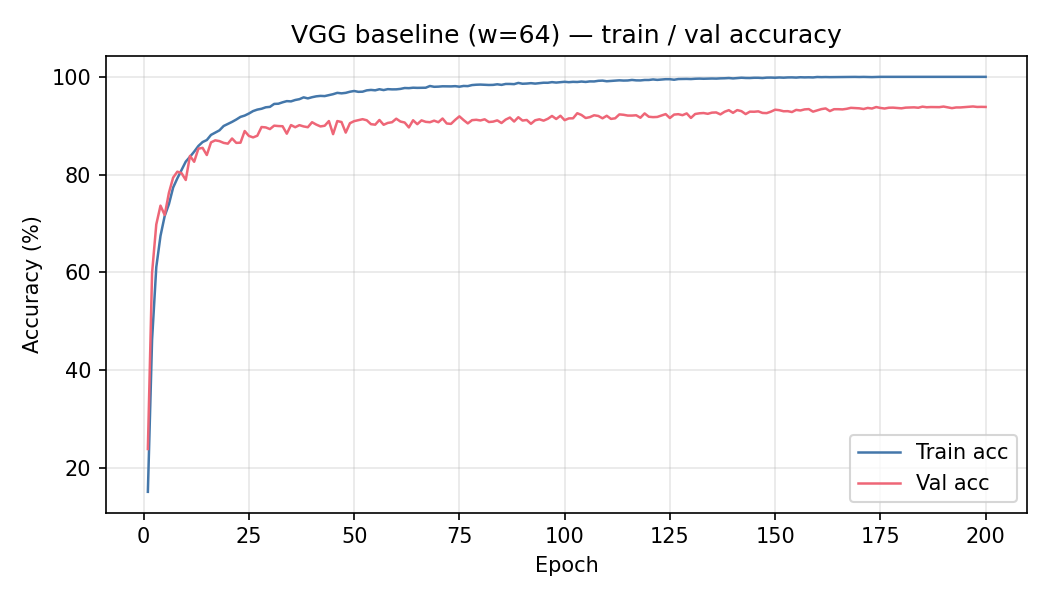
\includegraphics[width=0.58\linewidth]{vgg_baseline_train_val.png}
  \caption{\grade{E} VGG 训练/验证曲线（$w{=}64$）。}
  \label{fig:vgg}
\end{figure}

\subsection{\grade{B/A} FLOPs 对齐 block 对比}
\label{sec:ba}

表~\ref{tab:tier}（核心 RQ1）。\textbf{分析：}(1) 三档 test 均为 VGG 最高。(2) 中档 DW 在 279.6M FLOPs（约 VGG 的 90\%）下达 92.18\%，为全文最佳效率点。(3) CN 每档低 1.2--3.2 pt；高档 462M FLOPs 仍仅 90.12\%，低于中档 VGG。(4) VGG 从 $w{=}64$ 增至 $w{=}80$ 反而降点，可能存在大 width 过拟合。

\begin{table}[t]
  \caption{三档 FLOPs 对齐（val / test \%）。}
  \label{tab:tier}
  \centering
  \footnotesize
  \begin{tabular}{@{}llrrr@{}}
    \toprule
    档位 & 模型(width) & FLOPs & Val & Test \\
    \midrule
    低 & VGG(48) & 175.1M & 92.58 & \textbf{92.05} \\
    低 & DW(128) & 152.1M & 92.42 & 90.86 \\
    低 & CN(32) & 122.1M & 89.80 & 88.85 \\
    中 & VGG(64) & 309.5M & 93.92 & \textbf{92.78} \\
    中 & DW(175) & 279.6M & 92.46 & 92.18 \\
    中 & CN(52) & 309.2M & 90.70 & 90.34 \\
    高 & VGG(80) & 481.9M & 93.40 & \textbf{92.46} \\
    高 & DW(224) & 453.4M & 92.88 & 92.15 \\
    高 & CN(64) & 462.4M & 91.40 & 90.12 \\
    \bottomrule
  \end{tabular}
\end{table}

\begin{figure}[t]
  \centering
  \begin{subfigure}[t]{0.48\linewidth}
    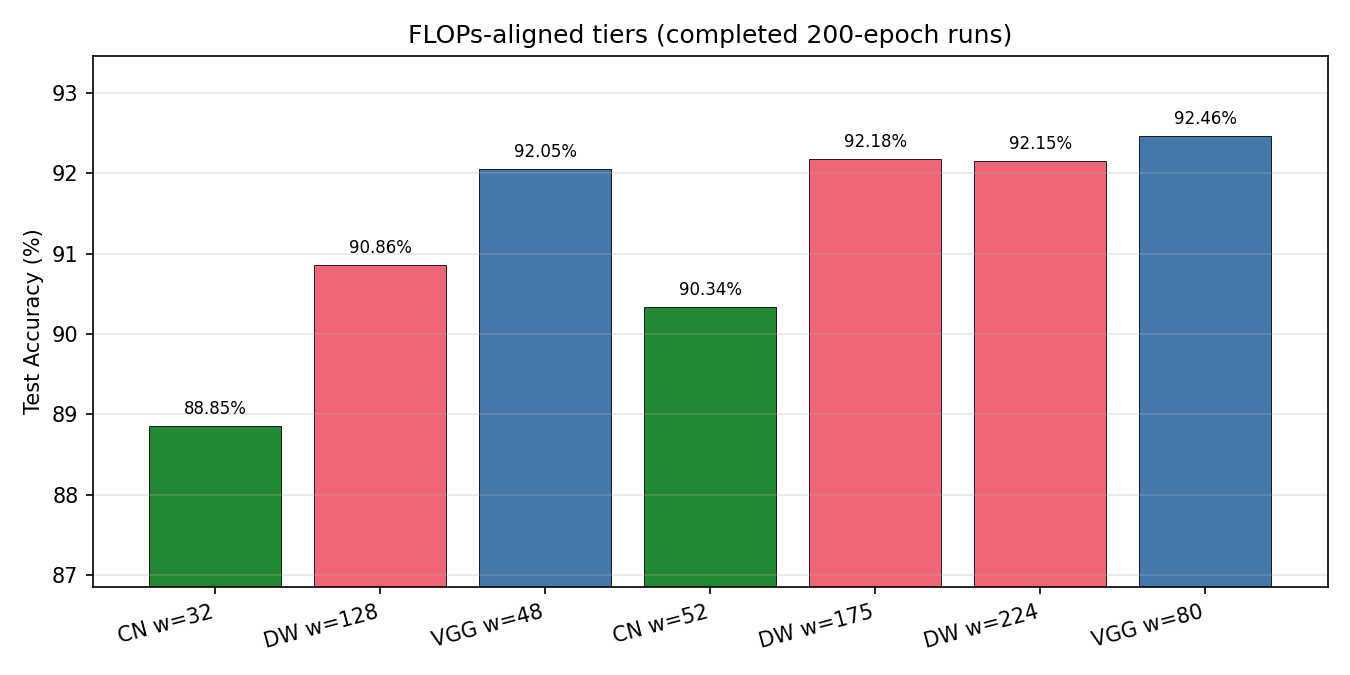
\includegraphics[width=\linewidth]{tier_test_accuracy.png}
    \caption{三档 test}
  \end{subfigure}\hfill
  \begin{subfigure}[t]{0.48\linewidth}
    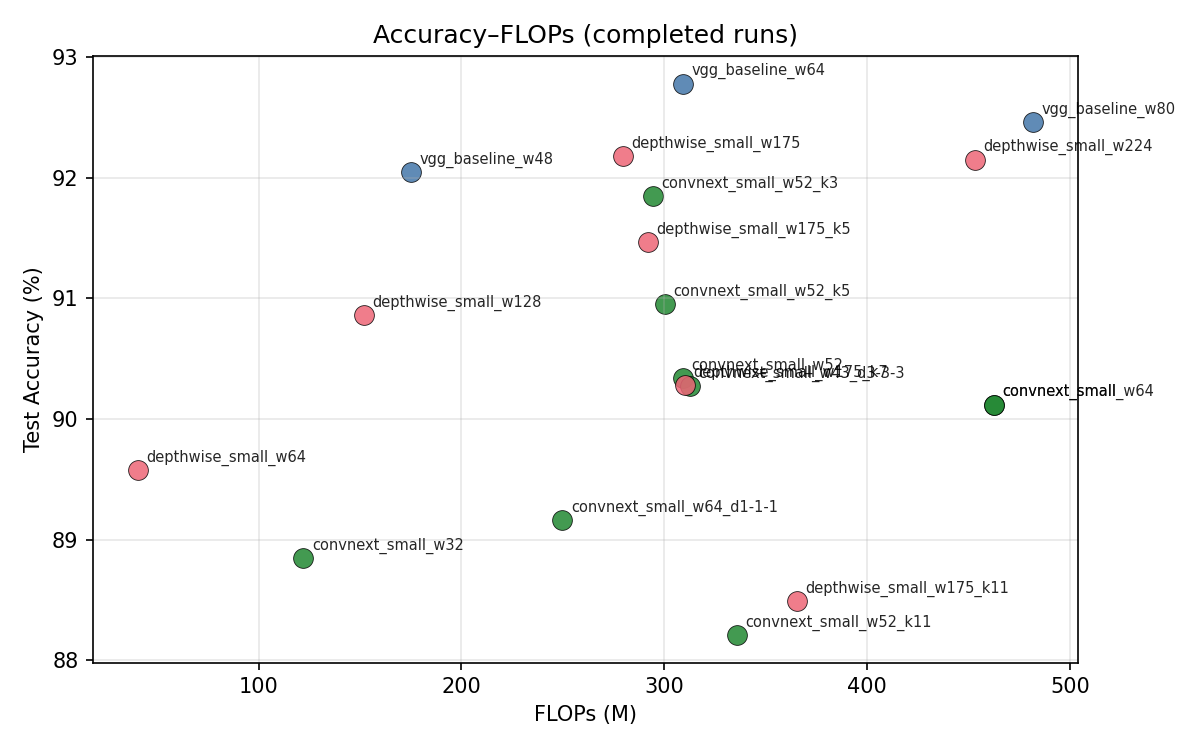
\includegraphics[width=\linewidth]{pareto_accuracy_flops.png}
    \caption{Pareto}
  \end{subfigure}
  \caption{\grade{B/A} 档位对比与精度--FLOPs Pareto。}
  \label{fig:main}
\end{figure}

\subsection{\grade{B/A} Width 缩放（\grade{D/C}）}

图~\ref{fig:width}：同族加宽一般提升 test 并增加 FLOPs；跨族比较时 VGG 在 175--310M 领先。表~\ref{tab:marginal}：VGG 在 $w{=}64$ 达峰；DW 从低$\to$中档边际收益最高（+1.04 pt/100M FLOPs）；CN 加宽有收益但绝对精度仍低于 VGG/DW。

\begin{table}[t]
  \caption{边际 test 收益（pt / 100M FLOPs）。}
  \label{tab:marginal}
  \centering
  \scriptsize
  \begin{tabular}{@{}llrrr@{}}
    \toprule
    族 & 对比 & $\Delta$FLOPs & $\Delta$test & 边际 \\
    \midrule
    VGG & $w{=}48{\to}64$ & +134M & +0.73 & +0.54 \\
    VGG & $w{=}64{\to}80$ & +172M & $-$0.32 & $-$0.19 \\
    DW & $w{=}128{\to}175$ & +127M & +1.32 & +1.04 \\
    DW & $w{=}175{\to}224$ & +174M & $-$0.03 & $-$0.02 \\
    CN & $w{=}32{\to}52$ & +187M & +1.49 & +0.80 \\
    CN & $w{=}52{\to}64$ & +153M & $-$0.22 & $-$0.14 \\
    \bottomrule
  \end{tabular}
\end{table}

\begin{figure}[t]
  \centering
  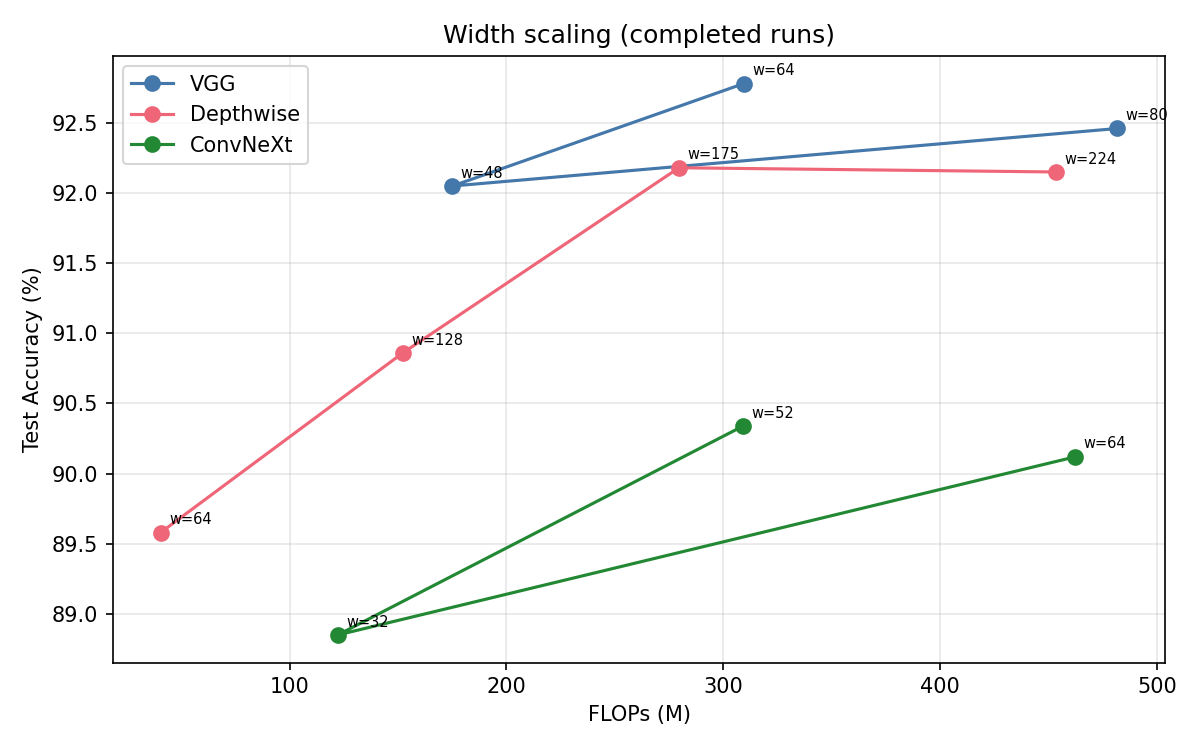
\includegraphics[width=0.68\linewidth]{width_scaling_accuracy_flops.png}
  \caption{各族 width 缩放曲线。}
  \label{fig:width}
\end{figure}

\subsection{\grade{B/A} Kernel 消融}

固定 CN $w{=}52$、DW $w{=}175$，扫描 $k{\in}\{3,5,7,11\}$（表~\ref{tab:kernel}，图~\ref{fig:kernel}）。CN：91.85$\to$90.95$\to$90.34$\to$88.21\%。DW：92.18$\to$91.47$\to$90.28$\to$88.49\%；$k{=}11$ 较 $k{=}3$ 降 \textbf{3.69 pt}。\textbf{RQ2（kernel）：}缩小至 $k{=}3$ 最优；增大 $k$ 为负边际收益。

\begin{table}[t]
  \caption{Kernel 扫描（test \%）。$^\dagger$：档位默认。}
  \label{tab:kernel}
  \centering
  \footnotesize
  \begin{tabular}{@{}crrrr@{}}
    \toprule
    $k$ & CN & DW & CN FLOPs & DW FLOPs \\
    \midrule
    3 & \textbf{91.85} & \textbf{92.18}$^\dagger$ & 294M & 280M$^\dagger$ \\
    5 & 90.95 & 91.47 & 300M & 292M \\
    7 & 90.34$^\dagger$ & 90.28 & 309M & 310M \\
    11 & 88.21 & 88.49 & 336M & 366M \\
    \bottomrule
  \end{tabular}
\end{table}

\begin{figure}[t]
  \centering
  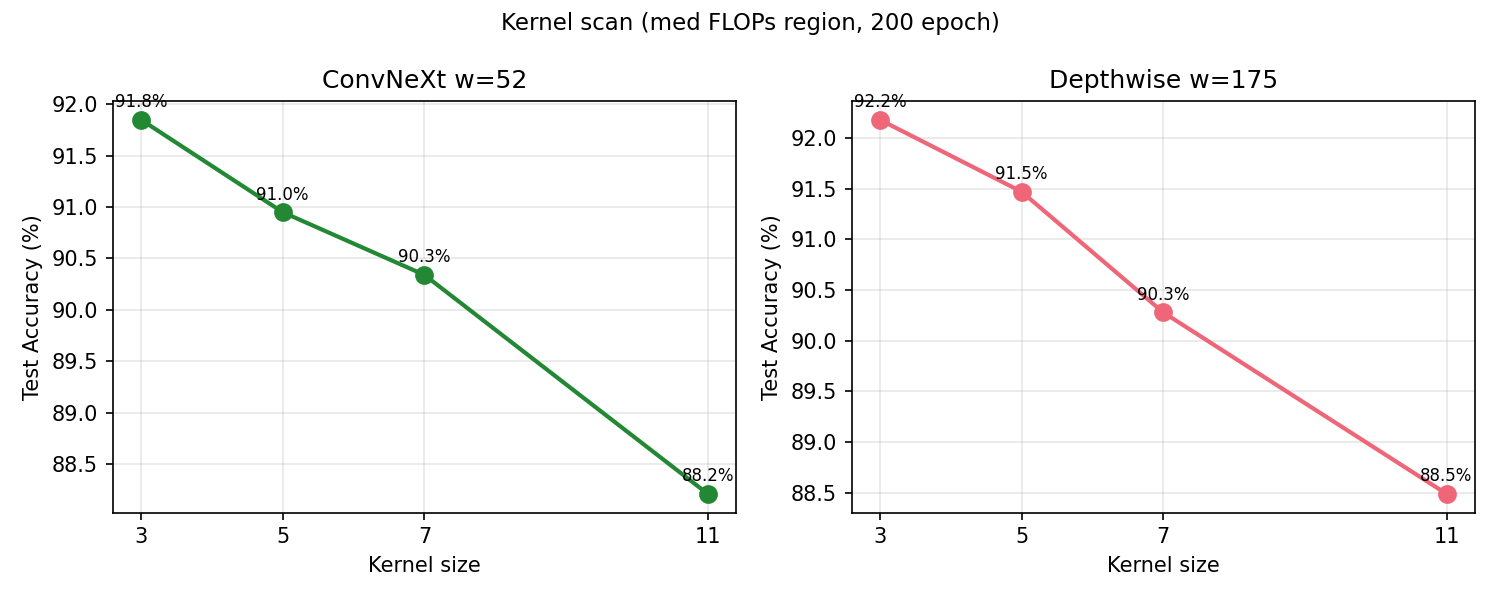
\includegraphics[width=0.55\linewidth]{kernel_scan_test_accuracy.png}
  \caption{Kernel 扫描曲线。}
  \label{fig:kernel}
\end{figure}

\subsection{\grade{B/A} Depth 与 Pareto 要点}

表~\ref{tab:depth}：浅层 $(1,1,1)$ 补训后 test 89.16\%；深层 $(3,3,3)$ 为 90.27\%，但仍低于 VGG $w{=}48$（175M，92.05\%）。表~\ref{tab:pareto}：非支配最高点仍为 \texttt{vgg\_w64}。

\begin{table}[t]
  \caption{ConvNeXt depth 变体（200 epoch）。}
  \label{tab:depth}
  \centering
  \footnotesize
  \begin{tabular}{@{}llrrrr@{}}
    \toprule
    depths & width & FLOPs & Val & Test & 说明 \\
    \midrule
    (2,2,2) & 64 & 462.4M & 91.40 & 90.12 & 默认 \\
    (2,2,2) & 52 & 309.2M & 90.70 & 90.34 & 中档 \\
    (1,1,1) & 64 & 249.8M & 90.90 & 89.16 & 补训 \\
    (3,3,3) & 43 & 312.9M & 91.08 & 90.27 & 深层 \\
    \bottomrule
  \end{tabular}
\end{table}

\begin{table}[t]
  \caption{代表性 Pareto 点（按 test 排序）。}
  \label{tab:pareto}
  \centering
  \scriptsize
  \begin{tabular}{@{}lrr@{}}
    \toprule
    run & FLOPs & Test \\
    \midrule
    vgg\_w64 & 309.5M & \textbf{92.78\%} \\
    vgg\_w48 & 175.1M & 92.05\% \\
    dw\_w175 & 279.6M & 92.18\% \\
    cn\_w52\_k3 & 294.3M & 91.85\% \\
    cn\_w52\_k11 & 336.1M & 88.21\% \\
    \bottomrule
  \end{tabular}
\end{table}

\begin{figure}[t]
  \centering
  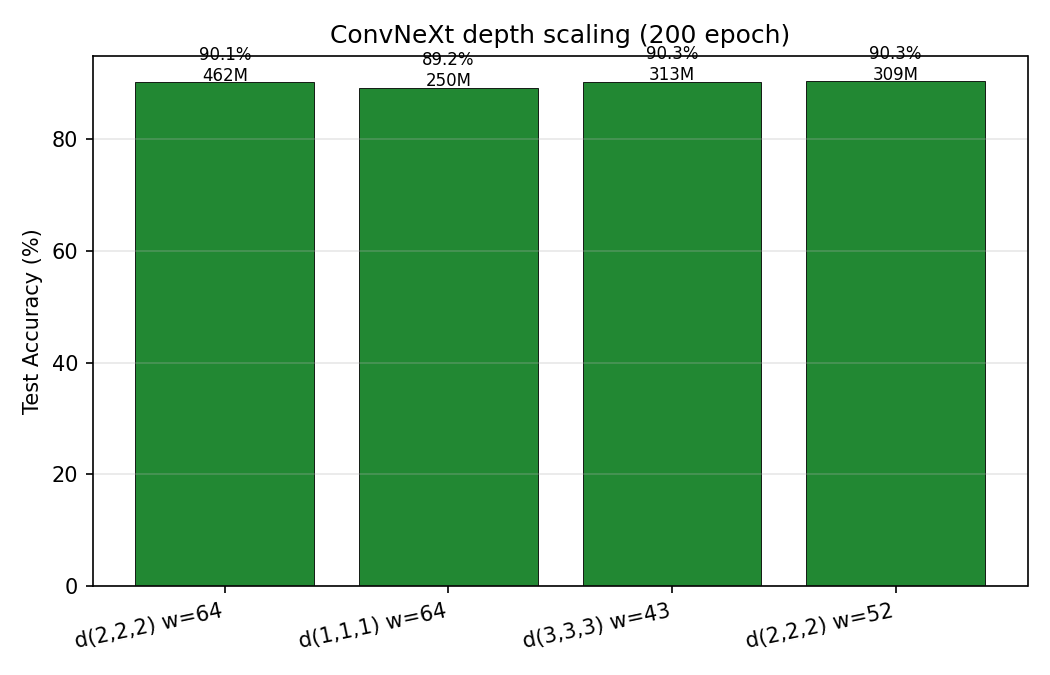
\includegraphics[width=0.55\linewidth]{depth_scan_test_accuracy.png}
  \caption{Depth 变体对比。}
  \label{fig:depth}
\end{figure}

\section{讨论与结论}
\label{sec:conc}

\subsection{RQ1 与 RQ2 的回答}

\textbf{RQ1（否）。}匹配 FLOPs 后 CN 未超过 VGG：低档差 3.20 pt、中档 2.44 pt、高档 2.34 pt。CN 最优（$k{=}3$，91.85\%）仍低于中档 VGG 0.93 pt。现代 block 未改善 CIFAR-10 上的 accuracy--FLOPs 权衡。

\textbf{RQ2。}最大正收益来自 \textbf{block 类型}（VGG $>$ DW $>$ CN）与 \textbf{DW 的 width}（低$\to$中）。\textbf{增大 kernel} 对 CN/DW 均为负收益。\textbf{depth} 仅改变 CN 内部排序。

\subsection{架构族对比}

\begin{table}[t]
  \caption{三族 block 在 CIFAR-10 上的定位（本实验）。}
  \label{tab:arch}
  \centering
  \footnotesize
  \begin{tabular}{@{}lccc@{}}
    \toprule
    族 & 精度 & 效率 & 建议 \\
    \midrule
    VGG+BN & 最高 & 中 & \textbf{默认首选} \\
    深度可分离 & 接近 VGG & 高 & 算力受限部署 \\
    ConvNeXt & 偏低 & 中 & 不建议照搬至 $32{\times}32$ \\
    \bottomrule
  \end{tabular}
\end{table}

三次池化后特征图约 $4{\times}4$；$k{=}11$ 易过平滑或放大边界伪影，ImageNet 式大核设计难以直接迁移。

\subsection{设计规则与总结论}

\begin{enumerate}[label=(\roman*)]
  \item 低 FLOPs（$<{\sim}180$M）：VGG $w{=}48$（92.05\%）；否则 DW $w{=}128$。
  \item 中 FLOPs（$\sim$280--330M）：VGG $w{=}64$（92.78\%）；算力敏感用 DW $w{=}175$（92.18\%）。
  \item 高 FLOPs：相对 $w{=}64$ 无收益；不建议加宽至 $w{=}80$。
  \item Kernel：保持 $k{=}3$；避免 $k{\geq}7$。
  \item CN depth：优先 $(2,2,2)$ 或 $(3,3,3)$。
\end{enumerate}

我们完成 17/17 次 200-epoch 实验。\textbf{VGG 为 Pareto 最优族}；\textbf{深度可分离}为最佳效率折中；\textbf{ConvNeXt 式大核堆叠}在公平比较下不足以证明算力价值。

\textbf{局限性：}单一 seed；静态 FLOPs；未测 GPU 延迟/能耗；MixUp/AMP 关闭。

\begin{ack}
  感谢 DD2424 课程组。分工：施博艺（模型 block）；朱璞皓（FLOPs、Pareto、图表）；龚金烨（训练管线与实验执行）。
\end{ack}

\bibliographystyle{plainnat}
\bibliography{references}

\end{CJK}
\end{document}
